\documentclass[12pt]{article}

\usepackage{sbc-template}
\usepackage[utf8]{inputenc}
\usepackage[T1]{fontenc}

\usepackage{graphicx,url}
\usepackage{amsmath,amssymb}
\usepackage{bm} % bold math

\usepackage{microtype}
\usepackage{booktabs}
\usepackage{dblfloatfix}
\usepackage{multirow}
\usepackage[section]{placeins}
\usepackage{float}
\makeatletter
\AddToHook{begindocument/before}[normalsfcodes-init]{%
  \global\let\normalsfcodes\@empty
}
\makeatother
\usepackage[english]{babel}
\usepackage[hidelinks]{hyperref}

\usepackage{tabularx}
\newcolumntype{H}{>{\setbox0=\hbox\bgroup}c<{\egroup}@{}} %coluna invisivel

\title{Comparing Lexical, Static-Embedding, and Contextual Drift Signals in Brazilian Portuguese Political Discourse}

\usepackage{subfigure}

\author{}
\address{}

% \author{Jo\~{a}o Victor M. Correa\inst{1} \and
%         Renato Moraes Silva\inst{1}}

% \address{Interinstitutional Center for Computational Linguistics (NILC)\\
%          Institute of Mathematics and Computer Science\\
%          University of S\~{a}o Paulo (USP), S\~{a}o Carlos, Brazil\\
% \email{victormcorrea@usp.br, renatoms@icmc.usp.br}
% }

\begin{document}

\maketitle

\begin{abstract}
The shift in political discourse often reflects deeper societal changes, but quantifying how specific terms evolve semantically over decades remains a significant challenge for computational linguistics. In this study, we compare three families of diachronic drift signals in Brazilian Portuguese
political discourse: a lexical-profile baseline based on TF-IDF, a static
embedding pipeline based on slice-specific Word2Vec models with Orthogonal
Procrustes alignment, and a contextual analysis based on a Portuguese BERT
checkpoint. %The study uses the floor subset of BrPoliCorpus, covering 24 yearly slices from 2000 to 2023 with 428{,}366 speeches and 63.0 million retained tokens after preprocessing. To make the methods directly comparable, we build a shared panel of 55 lemmas containing method-specific drift candidates, stable controls, and theory seeds. 
Using a BrPoliCorpus subset (428k speeches from 2000-2023), to make the methods directly comparable, we build a shared panel of 55 lemmas containing method-specific drift candidates, stable controls, and theory seeds. 
The resulting comparison shows strong disagreement between the
lighter baselines, with Spearman correlation of $-0.54$ and zero overlap in their
top 15 terms, while contextual BERT remains moderately closer to Word2Vec than
to TF-IDF. A filtered contextual panel reduces stable-control leakage and
highlights terms such as ``\textit{bloqueio}'', ``\textit{sal\'ario}'',
``\textit{interven\c{c}\~ao}'', and ``\textit{elei\c{c}\~ao}''. Rather than treating
one detector as externally validated ground truth, we frame the study as an
exploratory comparison of complementary drift sensitivities, interpretability,
and computational cost in Brazilian Portuguese political discourse.
\end{abstract}

\section{Introduction}
\label{sec:introduction}

% Political discourse is a productive setting for diachronic NLP because shifts in agenda, coalition structure, and policy framing leave traces in lexical choice and word usage over time. 
The language of politics reflects historical change, as shifts in ideological agendas, coalition structures, and policy framing become observable in patterns of lexical choice and word usage over time. However, manually analyzing large-scale and evolving patterns in political discourse is challenging. Diachronic natural language processing (NLP) methods offer promising avenues for analysis. Among these, distributional models can capture some of these movements at scale, but different modeling choices foreground different aspects
of change
\cite{hamilton-etal-2016-diachronic,kutuzov-etal-2018-diachronic,tahmasebi-etal-2021-computational}.
In political corpora the situation is especially complex, since a term may drift
because of a new policy referent, a rhetorical reframing, a shift in
collocational profile, or a reorganization of discourse coalitions, and none of
these mechanisms reduces neatly to a single lexical sense change.

This complexity carries over to evaluation, where shared-task benchmarks have
improved comparability in lexical semantic change
detection~\cite{schlechtweg-etal-2020-semeval} but curated external labels
remain scarce, especially outside the few languages and corpora covered by
standard tasks. Distributional pipelines can also react to temporal artifacts,
alignment noise, and other confounds when outputs are read too
literally~\cite{dubossarsky-etal-2019-timeout}. Without externally validated
ground truth, the central question becomes not which detector is ``correct''
but what each detector appears to capture when applied to the same political
timeline.

This question is timely for Brazilian Portuguese. Large-scale political corpora
such as BrPoliCorpus \cite{lima-lopes-2025-brpolicorpus} are only now becoming
available, yet comparative drift studies that place multiple detection families
side by side on the same Portuguese political material remain rare. We use the
floor subset of BrPoliCorpus, which covers 24 yearly slices of Chamber speeches
from 2000 to 2023, and compare a TF-IDF lexical-profile baseline, a
slice-specific aligned Word2Vec pipeline, and a contextual BERT stage, all
scored on a shared comparison panel of 55 lemmas. The paper addresses the following questions: 

\begin{enumerate}
    \item How strongly do the methods agree on the same lemmas? 

    \item Which candidates remain method-specific?

    \item Does the higher-cost contextual
stage add enough interpretive value to justify its expense?
\end{enumerate}

The comparisons conducted to address these research questions
fill a descriptive gap in Portuguese, where published multi-method drift
analyses remain much scarcer than in the better-studied English-centered
literature.

\section{Related Work}
\label{sec:related_work}

Distributional semantic change detection has evolved from co-occurrence
comparisons to aligned static embeddings and then to contextual
representations~\cite{kutuzov-etal-2018-diachronic,tahmasebi-etal-2021-computational}.
Among static approaches, slice-specific Word2Vec models aligned with Orthogonal
Procrustes have been shown to recover known historical shifts and reveal
statistical regularities of
change~\cite{hamilton-etal-2016-diachronic}.
Such embeddings remain attractive because they are efficient and produce
interpretable neighborhood movements, but they compress all usages of a word
into a single vector, blurring cases in which older and newer usages coexist.

Evaluation remains the harder problem. Standardized shared tasks have improved
comparability \cite{schlechtweg-etal-2020-semeval}, yet many real-world studies
still operate without external semantic ground truth, and apparent change can
emerge from temporal referencing, alignment noise, or genre shifts rather than
from semantic drift alone \cite{dubossarsky-etal-2019-timeout}. This concern
motivates the stable controls and agreement analysis in the present work.

Contextual models offer a partial response to the aggregation problem.
BERT-style representations encode token-level usages and can surface variation
that static spaces smooth over
\cite{giulianelli-etal-2020-analysing,devlin-etal-2019-bert}.
Scalable contextual methods that improve interpretability have also been
proposed \cite{montariol-etal-2021-scalable}, and pre-trained Portuguese
checkpoints such as BERTimbau \cite{souza-etal-2020-bertimbau} have made
contextual analysis feasible for Portuguese NLP\@. We place contextual BERT
beside TF-IDF and aligned Word2Vec on the same
political panel so that agreement, disagreement, and computational tradeoffs
can be examined directly.

Diachronic analysis of political language has gained traction through
parliamentary corpora. The study of \cite{hofmann-etal-2020-comparing}
compared lexical usage in Austrian political discourse across time, but
comparable multi-method studies on Brazilian Portuguese political speech remain
scarce. Existing Portuguese diachronic
resources~\cite{osorio-cardoso-2025-historical} have focused primarily on
historical and literary material rather than political discourse, leaving a
gap that BrPoliCorpus \cite{lima-lopes-2025-brpolicorpus} now fills with the
scale needed for controlled comparative work.

\section{Corpus and Experimental Setup}
\label{sec:data_setup}


The experiments use the floor subset of BrPoliCorpus
\cite{lima-lopes-2025-brpolicorpus}, which contains Brazilian Chamber floor
speeches from 2000 to 2023 organized into 24 yearly slices. A growing number of diachronic Portuguese resources are now
available~\cite{osorio-cardoso-2025-historical}, ranging from syntactically
annotated literary collections such as the Tycho Brahe Parsed
Corpus~\cite{galves-faria-2017-tycho} to large multi-genre repositories such
as the Corpus do
Portugu\^es~\cite{davies-ferreira-2006-corpusdoportugues}. These resources
target historical-linguistic research across broad periods rather than
domain-specific political analysis with continuous yearly slices. Within
BrPoliCorpus itself, the inaugural-speech subset reaches back to 1889 but
contains only 35 documents, too few for stable distributional estimation. The
floor subset offers the largest contiguous yearly coverage (428{,}366 speeches
across 24 slices), a uniform parliamentary register, and exact date metadata,
making it the most suitable segment for a year-by-year comparative drift study
in the political domain.

\subsection{Preprocessing}

Raw speeches are tokenized and tagged with
\texttt{spaCy} (\texttt{pt\_core\_news\_sm}). We retain nouns, verbs, and
adjectives, exclude proper nouns, remove stopwords, punctuation, and numeric
tokens, and keep only tokens with at least two characters. All text is
lowercased with accents preserved. Each token is then mapped to its lemma form,
producing the \texttt{content\_lemma} representation used by all three methods.
After preprocessing, the corpus retains 428{,}366 speeches and
63{,}036{,}642 tokens across 225{,}484 unique lemmas.
Table~\ref{tab:dataset_summary} summarizes the corpus totals and the quartile
structure of yearly variation.

\subsection{Candidate Eligibility}

A lemma enters the scored vocabulary only if
it appears at least 50 times per slice, in at least 5 documents per slice, and
in at least 80\% of the 24 slices. These thresholds were fixed as practical
corpus-stability defaults rather than tuned to optimize any particular method.
The frequency floor ensures sufficient token mass for reliable embedding
training in each yearly slice; the document-dispersion requirement prevents a
single speaker or parliamentary session from inflating a lemma's apparent
salience; and the slice-presence constraint restricts attention to lemmas that
are genuinely diachronic rather than episodic. Drift and stable-control
candidates are further restricted to dominant part-of-speech classes (nouns and
adjectives), and a small set of procedural high-frequency terms is excluded.
These filters reduce the scored vocabulary to 3{,}221 lemmas for the two
cheaper methods.

Yearly document counts range from 3{,}041 to 26{,}868 (median 16{,}752) and
retained token volume from 630K to 4.2M (median 2.6M). Document volume is high
throughout, but token and vocabulary variation across slices motivates the
frequency and slice-presence controls described above.

\begin{table*}[!htb]
    \centering
    \footnotesize
    \setlength{\tabcolsep}{5pt}
    \renewcommand{\arraystretch}{1.08}
    \caption{Corpus summary for the BrPoliCorpus floor subset. Yearly slice statistics are
    reported as the 25th percentile (Q1), median, and 75th percentile (Q3) across the 24 yearly files; token and character
    counts are shown in millions.}
    \label{tab:dataset_summary}
%
\begin{tabularx}{\textwidth}{@{}c c l 
>{\raggedleft\arraybackslash}X 
>{\raggedleft\arraybackslash}X
>{\raggedleft\arraybackslash}X
>{\raggedleft\arraybackslash}X@{}}
\toprule

\multirow{2}{*}{Period} & \multirow{2}{*}{Slices} & \multirow{2}{*}{Measure} & \multirow{2}{*}{Corpus total} & \multicolumn{3}{c}{Yearly slices} \\ \cmidrule(lr){5-7}

 &  &  &  & Q1 & Median & Q3 \\
\midrule

\multirow{4}{*}{2000--2023} 
& \multirow{4}{*}{24} 
& Speeches 
& 428{,}366 
& 14{,}648 
& 16{,}752 
& 21{,}987 \\

& & Tokens 
& 63.0M 
& 2.00 
& 2.62 
& 3.45 \\

& & Characters 
& 538.5M 
& 16.9 
& 22.3 
& 29.7 \\

& & Lemmas 
& 225{,}484 
& 39{,}456 
& 50{,}269 
& 58{,}637 \\

\bottomrule
\end{tabularx}

\end{table*}

\FloatBarrier

\section{Methodology}
\label{sec:methodology}

Figure~\ref{fig:study_design} summarizes the workflow, which was designed for
this study rather than adopted from a single prior work. Each
component, from TF-IDF lexical profiles and slice-aligned Word2Vec to
contextual BERT inspection, is individually grounded in the
literature~\cite{hamilton-etal-2016-diachronic,giulianelli-etal-2020-analysing},
but their orchestration into a cost-aware comparative pipeline is ours. The
sequence follows a deliberate logic in which two cheaper baselines first
screen the full scored vocabulary, and their method-led candidates are then
combined with
stable controls and theory seeds to create the shared panel used for
contextual inspection and agreement analysis. This design concentrates the
more expensive contextual stage on the subset where inter-method disagreement
makes adjudication most informative.

\subsection{TF-IDF Baseline}

For each eligible lemma we compute a TF-IDF vector
across yearly slices using smoothed inverse-document frequency. Drift is
measured as the mean absolute change in TF-IDF weight between adjacent slices.
This captures shifts in lexical salience, reflecting how central a term becomes
to each year's agenda, without relying on distributional neighborhoods.

\subsection{Word2Vec Baseline}

We train independent skip-gram models per yearly
slice (300 dimensions, window~5, 5 negative samples, minimum count~5, 5 epochs,
2 replicates with different seeds) and align them into a common space with
Orthogonal Procrustes over the top 20{,}000 anchor words
\cite{hamilton-etal-2016-diachronic}. Drift is the mean cosine distance between
a lemma's aligned vectors in consecutive slices, averaged over replicates. This
captures persistent neighborhood reorganization.

\subsection{Contextual BERT}

We embed sampled in-context occurrences with a Portuguese
BERT checkpoint (BERTimbau Large~\cite{souza-etal-2020-bertimbau}),
extracting hidden-state layers $-1$ and~$-4$. For each lemma and slice, up to 64 occurrences are sampled within a
48-token context window; the contextual drift score is the mean cosine distance
between slice-level centroid embeddings in consecutive slices. The agreement
layer keeps layer~$-1$ as the preferred ranking and uses layer~$-4$ as a
robustness view.

\subsection{Shared Comparison Panel}

Rather than compare unrestricted vocabularies, we construct a shared panel of
55~lemmas: 15 Word2Vec-led drift candidates, 15 TF-IDF-led drift candidates,
20~stable controls (lemmas ranked lowest by both cheap methods), and 5~theory
seeds drawn from prior work on Brazilian political vocabulary
(\textit{democracia}, \textit{corrup\c{c}\~ao}, \textit{reforma},
\textit{economia}, \textit{liberdade}). All three methods observe the same
candidate set, so disagreement reflects properties of the signal rather than
divergent vocabularies. The agreement layer derives pairwise rank correlations,
top-$k$ overlaps, stable-control leakage diagnostics, and a filtered contextual
ranking.

Figure~\ref{fig:method_agreement} visualizes the pairwise agreement structure,
while Figure~\ref{fig:overlap_rank_stats} summarizes overlap and
rank-distribution statistics.

\begin{figure}[!htb]
    \centering
    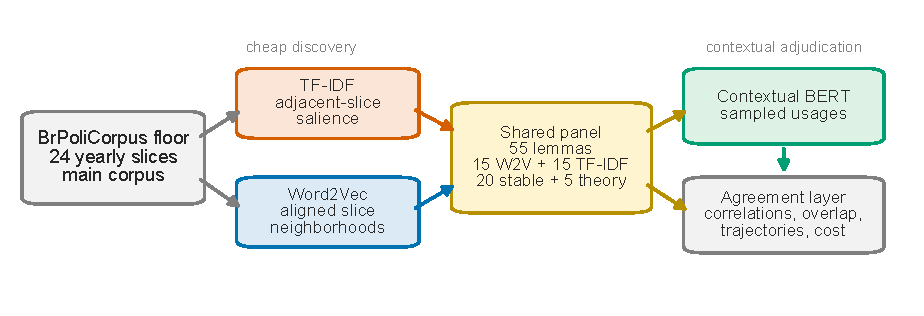
\includegraphics[width=0.86\linewidth]{figs/paper/figure_05_study_design.pdf}
    \caption{Comparative workflow. The two cheaper baselines nominate
    candidates; the shared panel combines those candidates with controls and
    theory seeds before contextual inspection and agreement analysis.}
    \label{fig:study_design}
\end{figure}

\section{Results}
\label{sec:results}

The two lighter baselines disagree strongly even after they are constrained to
the same candidate universe. On the shared panel, Word2Vec and TF-IDF reach
Spearman $\rho = -0.54$ ($p = 2.1 \times 10^{-5}$) and share zero terms in
their top 15 rankings. The preferred contextual layer partly mediates this
split without collapsing onto either baseline. Its correlation with Word2Vec is
$\rho = 0.21$ ($p = 0.128$) and with TF-IDF $\rho = 0.12$ ($p = 0.365$).
These positive associations are directionally informative but not strong enough
to justify treating contextual BERT as a substitute for either cheaper method.
Figure~\ref{fig:method_agreement} visualizes this pairwise rank structure.
Each panel plots the drift scores of the 55 lemmas under two methods, with
Spearman $\rho$ and $p$-values annotated. Panel~(A) reveals the strong
negative trend between Word2Vec and TF-IDF, where terms ranked highly by one
baseline tend to be ranked low by the other, confirming that they capture
fundamentally different facets of change. Panels~(B) and~(C) show that
contextual BERT draws partial support from both camps without collapsing onto
either, while Panel~(D) confirms that the two BERT extraction layers agree
closely with each other.

\begin{figure}[!htb]
    \centering
    
\includegraphics[width=1.0\linewidth]{figs/paper/figure_02_method_agreement.pdf}
    \caption{Agreement on the shared panel across TF-IDF, Word2Vec, and the
    preferred BERT layer; panel (D) compares BERT layers -4 and -1.
    Annotations report Spearman $\bm{\rho}$ and two-sided p-values.}
    \label{fig:method_agreement}
\end{figure}

\begin{figure}[!htb]
	\centering
	\subfigure[Performance evaluated in all words.\label{fig:dunn_allWords}]{
		\centering
		
\includegraphics[width=1.0\linewidth]{figs/paper/figure_02_method_agreement.pdf}
	}
	\quad
	\subfigure[Performance evaluated only in the OOV words.\label{fig:dunn_onlyOOVs}]{
		\centering
		
\includegraphics[width=1.0\linewidth]{figs/paper/figure_02_method_agreement.pdf}
	}
	\caption{Average rankings and critical differences calculated using the Bonferroni-Dunn
post-hoc test.\label{fig:statisticalAnalisys}}
     
\end{figure}


Overlap statistics and bucket-level rank distributions prove more informative
than raw top-$k$ lists alone. In the preferred BERT layer,
the top-15 overlap is 7 terms with Word2Vec and 6 terms with TF-IDF, whereas the
baseline-to-baseline overlap remains zero. Figure~\ref{fig:overlap_rank_stats} also
shows that selected drift terms are ranked significantly above stable controls by
Word2Vec and TF-IDF ($p < .001$ in both cases), while contextual BERT still
separates the groups but with weaker margins ($p = .008$). This pattern is
consistent with the filtered contextual panel, where BERT
provides useful adjudication but the raw contextual ranking still leaks some
stable controls and should not be treated as an unrestricted final list. The
two contextual extraction layers nevertheless agree strongly with each other
(Spearman $= 0.858$), so the broad comparative picture does not depend on a
single extraction depth. This high inter-layer agreement accords with findings
that mid-to-upper layers carry most of the semantic change signal, while the
final layer increasingly encodes surface-form information that can bias change
scores~\cite{laicher-etal-2021-explaining,cassotti-etal-2024-systematic}; the
stability between layers $-1$ and $-4$ in our setting suggests that
orthographic bias does not yet dominate, though it does not rule it out.

As a robustness check, we recomputed contextual scores using average pairwise
distance (APD)~\cite{giulianelli-etal-2020-analysing} instead of the centroid-based
metric. APD operates on all individual occurrence embeddings rather than on
slice-level centroids, giving equal influence to each usage regardless of
embedding magnitude. On the preferred layer, APD and centroid rankings
correlate at Spearman $\rho = 0.79$ ($p < 10^{-12}$), with 7 of 15 top terms
shared. The two metrics foreground different properties: APD promotes
high-frequency polysemous terms whose embedding clouds are broad (e.g.\
\textit{trabalho}, \textit{p\'ublico}), while the centroid metric favours
terms with coherent directional shifts (\textit{bloqueio},
\textit{sal\'ario}). Notably, the centroid metric separates method-nominated
drift candidates from stable controls more cleanly than APD ($p = .008$ vs.\
$p = .081$, Mann--Whitney). The strong overall correlation confirms that the
comparative conclusions are robust to the choice of contextual aggregation,
while the separation difference suggests that centroid distance is a less
noisy signal for this panel-based comparison.

\begin{figure}[!htb]
    \centering
    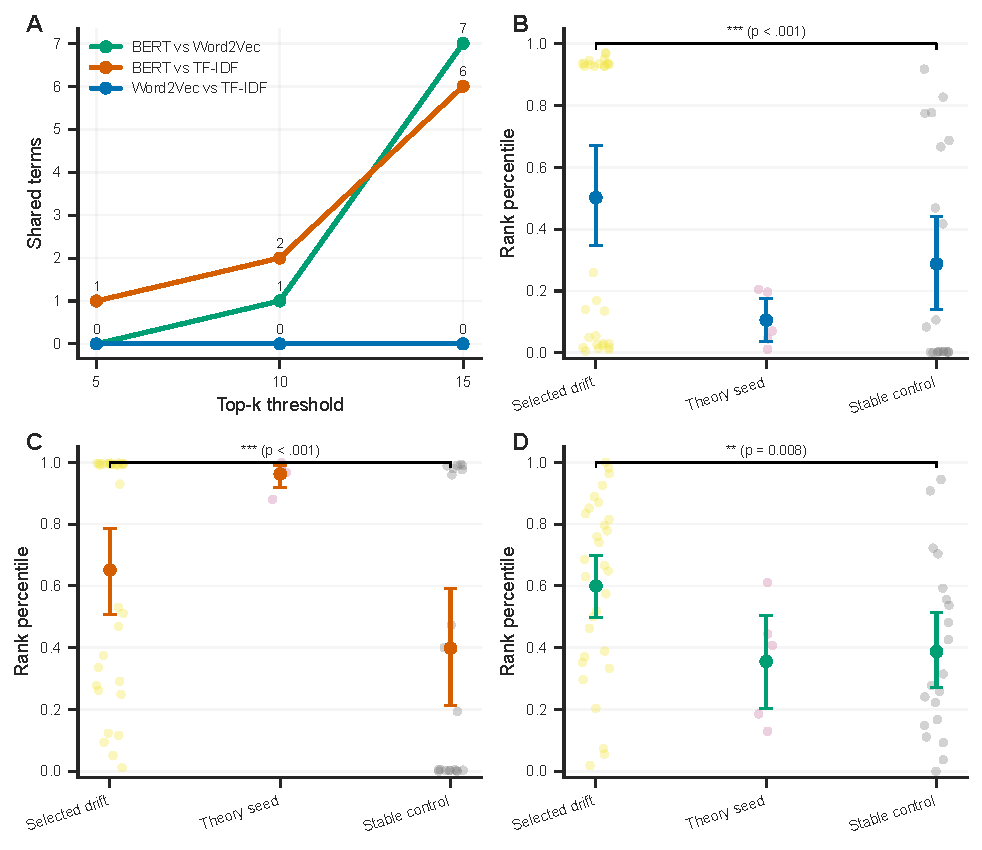
\includegraphics[width=0.90\linewidth]{figs/paper/figure_03_overlap_and_rank_statistics.pdf}
    \caption{Overlap and rank-distribution summaries on the shared comparison
    panel. Panel (A) traces top-$\bm{k}$ overlap; panels (B) through (D) compare
    rank-percentile distributions for selected drift terms, theory seeds, and
    stable controls.}
    \label{fig:overlap_rank_stats}
\end{figure}

\section{Discussion}
\label{sec:discussion}

Representative term trajectories show that the methods often disagree about
\emph{when} a term moves, not only whether it moves at all. Figure~\ref{fig:representative_trajectories}
illustrates four cases: a Word2Vec-led term with strong contextual support
(\textit{bloqueio}), a TF-IDF-led term with strong contextual support
(\textit{sal\'ario}), a theory seed whose contextual rank rises despite modest
static drift (\textit{reforma}), and a stable-control diagnostic term
(\textit{trabalho}) that reveals where contextual leakage remains.

\begin{figure}[!htb]
    \centering
    
\includegraphics[width=0.92\linewidth]{figs/paper/figure_04_representative_trajectories.pdf}
    \caption{Representative term trajectories across methods. Scores are
    standardized within term and method to emphasize temporal shape rather than
    absolute scale.}
    \label{fig:representative_trajectories}
\end{figure}

The disagreement itself is substantively informative, because each method
foregrounds a different facet of lexical change. TF-IDF is most sensitive to
lexical-profile reweightings, so a term whose salience rises in yearly agendas,
policy disputes, or formulaic framing can register as drifting even if its local
semantic neighborhood remains comparatively stable. Word2Vec, by contrast,
captures persistent neighborhood reorganization across slices. Contextual BERT
occupies an intermediate position and can support either a TF-IDF-led or a
Word2Vec-led candidate through its token-level representations, although the
stable-control leakage analysis shows that greater context sensitivity does not
automatically produce a cleaner unrestricted ranking.

The term-level evidence supports this interpretation. \textit{Sal\'ario}
behaves like a lexical-profile case with strong contextual support, suggesting
that changes in agenda prominence and usage framing are both at work.
\textit{Bloqueio} looks more like a neighborhood-displacement case in which the
contextual layer aligns with the embedding-led signal. \textit{Reforma}
illustrates a complementary pattern, since as a theory seed it displays
contextual differentiation despite ranking modestly in the cheaper methods. The
shared panel includes theory seeds and stable controls alongside method-led
drift terms to make such distinctions recoverable.

\begin{table}[!htb]
    \centering
    \footnotesize
    \caption{Method scope and relative computational cost. The cost column
    reports order-of-magnitude class
    and approximate multiplier relative to TF-IDF, measured on the same
    single-machine run; absolute wall-clock times will vary with hardware.}
    \label{tab:method_profile}
    \begin{tabularx}{\linewidth}{@{}l>{\raggedright\arraybackslash}Xl >{\raggedright\arraybackslash}X@{}}
        \toprule
        Method & Signal focus & Scope & Relative cost \\
        \midrule
        TF-IDF & Adjacent-slice salience shift & 3{,}221 lemmas & seconds ($1{\times}$) \\
        Word2Vec & Aligned neighborhood displacement & 3{,}221 lemmas & minutes (${\sim}56{\times}$) \\
        Contextual BERT & Usage divergence from sampled contexts & 55 lemmas / 82{,}461 occurrences & hours (${\sim}600{\times}$) \\
        \bottomrule
    \end{tabularx}
\end{table}

Table~\ref{tab:method_profile} quantifies the cost gap. TF-IDF runs in
seconds, Word2Vec in minutes at corpus scale, and contextual BERT is roughly
two orders of magnitude more expensive even after restriction to the 55-lemma
panel. Given the modest rank
correlations reported above, the current evidence does not support replacing the
cheaper methods with BERT but instead favours using contextual modeling
selectively as an adjudication layer when the disagreement is substantively
interesting.

\FloatBarrier

\section{Conclusion}
\label{sec:conclusion}

Returning to the research questions posed in the introduction, the evidence
supports three answers. First, regarding the strength of inter-method
agreement, TF-IDF and Word2Vec disagree strongly on the shared panel (Spearman
$\rho = -0.54$, zero top-15 overlap), and contextual BERT remains only weakly
correlated with either baseline ($\rho = 0.21$ with Word2Vec, $\rho = 0.12$
with TF-IDF), so the three families do not converge on a single ranking.
Second, regarding method-specific candidates, all 30 drift terms nominated by
the two cheaper methods are exclusive to one baseline; BERT partially bridges
this split by placing candidates from both camps among its top-ranked terms,
but it also retains some stable controls in high positions, so its raw ranking
should not be treated as an unrestricted candidate list. Third, regarding the
cost--benefit of the contextual stage, BERT provides useful adjudication when
inter-method disagreement is substantively interesting, as illustrated by
terms such as \textit{bloqueio}, \textit{sal\'ario}, and \textit{reforma}.
At roughly $600{\times}$ the cost of TF-IDF, though, the current evidence
favors using it selectively rather than as a replacement for the cheaper
methods. Taken
together, these results frame disagreement itself as part of the
contribution, suggesting that the three method families are sensitive to
different mixtures of lexical
salience, neighborhood displacement, and usage-level variation in Brazilian
Portuguese political discourse.

\section{Limitations}
\label{sec:limitations}

The primary evaluative limitation is that this paper does not claim external
semantic ground truth for BrPoliCorpus floor, so agreement and disagreement are
analyzed as comparative evidence rather than as proof that one detector is
correct. A second, methodological limitation is that the raw contextual ranking
still admits some stable controls near the top, even though the filtered
contextual list is useful for interpretation; contextual sensitivity does not
automatically yield a cleaner unrestricted candidate list. The choice of
contextual aggregation strategy also merits discussion. We report centroid-based
drift as the primary contextual metric and verify it against
APD~\cite{giulianelli-etal-2020-analysing,cassotti-etal-2024-systematic}
(Section~\ref{sec:results}); the strong correlation and the centroid metric's
tighter bucket separation support this choice, though APD captures
complementary embedding-cloud variance. Sense-based clustering
methods~\cite{montariol-etal-2021-scalable} were not attempted here. Finally,
yearly slicing is appropriate for a first comparative baseline but
compresses within-year shocks, campaign cycles, and short-lived institutional
disputes that may matter for political language.

Future work could address the evaluative gap through external annotation
or noisy supervision from labeled parliamentary datasets, though such resources
still require careful deduplication before serving as reliable comparison
targets. On the modeling side, adopting task-specialized
models such as
XL-LEXEME~\cite{cassotti-etal-2024-systematic}, exploring newer divergence
metrics~\cite{rachinskiy-schlechtweg-2025-rethinking}, and applying
orthographic-bias mitigation through subword
masking~\cite{laicher-etal-2021-explaining} would bring the contextual stage
closer to current best practices. A symbolic companion analysis using lexical
complexity or readability features could also help separate lexical-semantic
drift from rhetorical or stylistic change.

\section{Ethics Statement}
\label{sec:ethics}

The study analyzes public institutional political speech and reports only
aggregate corpus statistics, ranked lemmas, and usage-level comparative signals.
We do not profile individual speakers or infer private attributes. Even so,
political corpora encode unequal representation and occasionally harmful
rhetoric, so drift scores should not be read as normative judgments, evidence
of speaker intent, or standalone claims about social meaning. All outputs are
exploratory comparative signals whose interpretation depends on corpus
composition, preprocessing choices, and the distinction between lexical
salience, contextual variation, and broader discourse change.

\bibliographystyle{sbc}
\bibliography{bib/bib_main}

\end{document}
